This section describes the methodology that is proposed to be followed during the development of the project.

\subsection{Proposed Software Development Life Cycle}
The project will be developed as per the waterfall model\cite{waterfall} of the software development life cycle as depicted in Figure \ref{fig:sdlc}. The reason for choosing this model is the lack of sufficient time duration for agile and iterative methods, as well as very low chances of changes of requirements in the process of development. 

\begin{figure}[h]
	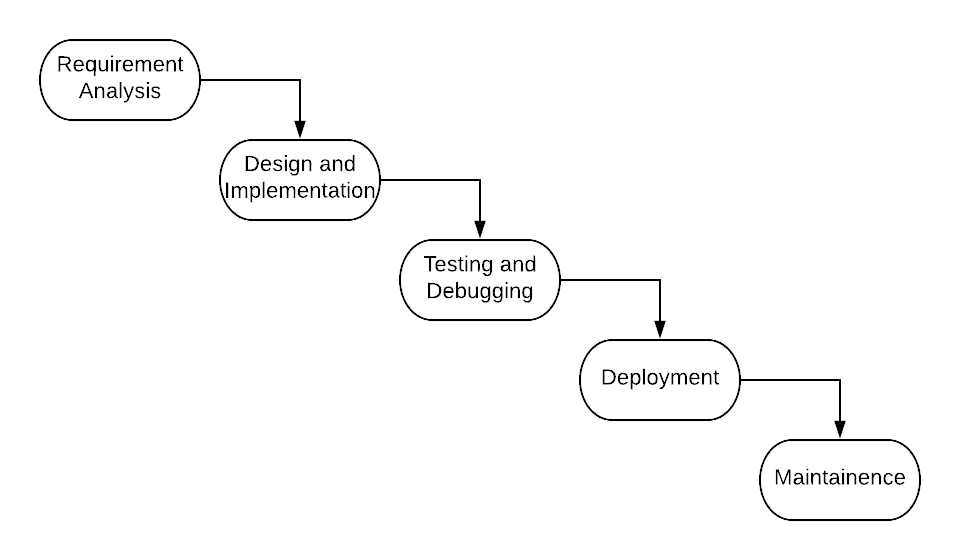
\includegraphics[width=\linewidth]{figures/sdlc.png}
	\centering
	\caption{Proposed software development life cycle}
	\label{fig:sdlc}
\end{figure}

The life cycle begins when the team collects and evaluates the requirements that will be expected from the application. The design and implementation phase will be to design and build both API services and client applications. By the end of this phase, a minimal viable product (MVP) will already have been constructed. In the testing and debugging phases, the quality control methods will be applied to both API and application. Finally, the application will be deployed to Docker containers at the end of the deployment phase. However, there might be slight modifications in the original waterfall model where the design and implementation may be changed slightly after the testing phase if seen as reasonable.

\subsection{Technical Architecture}
The application will be built upon the client-server web architecture, as illustrated in Figure \ref{fig:arch}.

\begin{figure}[H]
    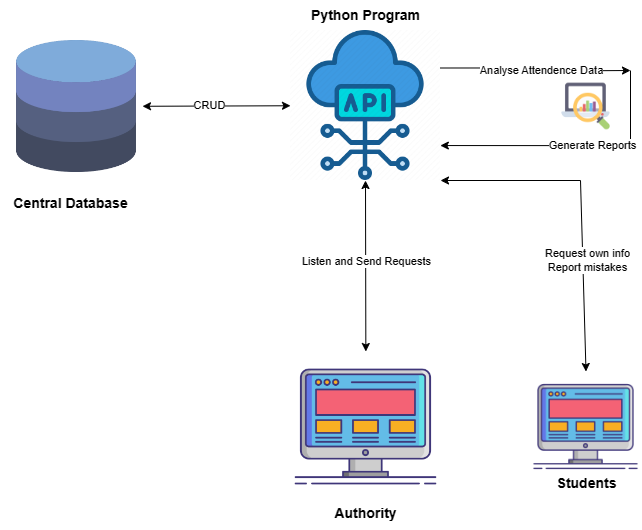
\includegraphics[width=\linewidth]{figures/architecture.png}
    \centering
    \caption{Proposed architecture of the application}
    \label{fig:arch}
\end{figure}

The architecture consists of a database that handles data storage and management. Python is responsible for handling Create, Read, Update, and Delete (CRUD) operations on the database. It also provides WebSocket communication capabilities to the client application.\\

The client application allows students to access their personal attendance information securely. Only authorized personnel, such as administrators or instructors, can access the entire dataset via the client application using WebSocket communication.\\

Python program acts as the intermediary between the client application and is also responsible for generating reports based on the attendance data. This communication ensures seamless integration and efficient report generation.\\

\begin{figure}[H]
    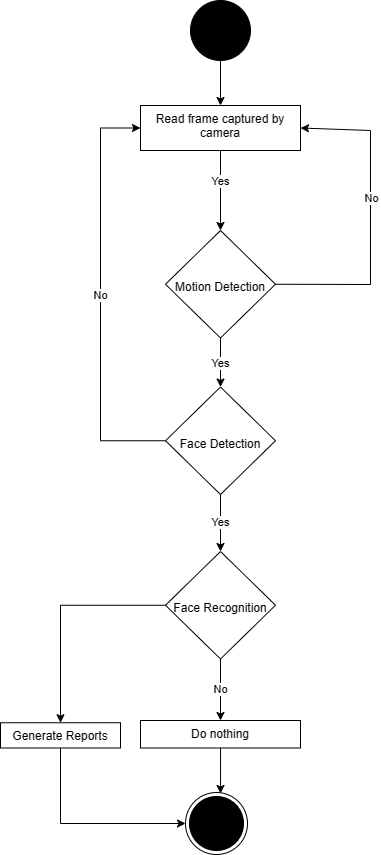
\includegraphics[width=0.6\linewidth]{figures/activity-diagram.png}
    \centering
    \caption{Activity Diagram\cite{yasmeensmart} of the application}
    \label{fig:activity}
\end{figure}

\begin{figure}[H]
    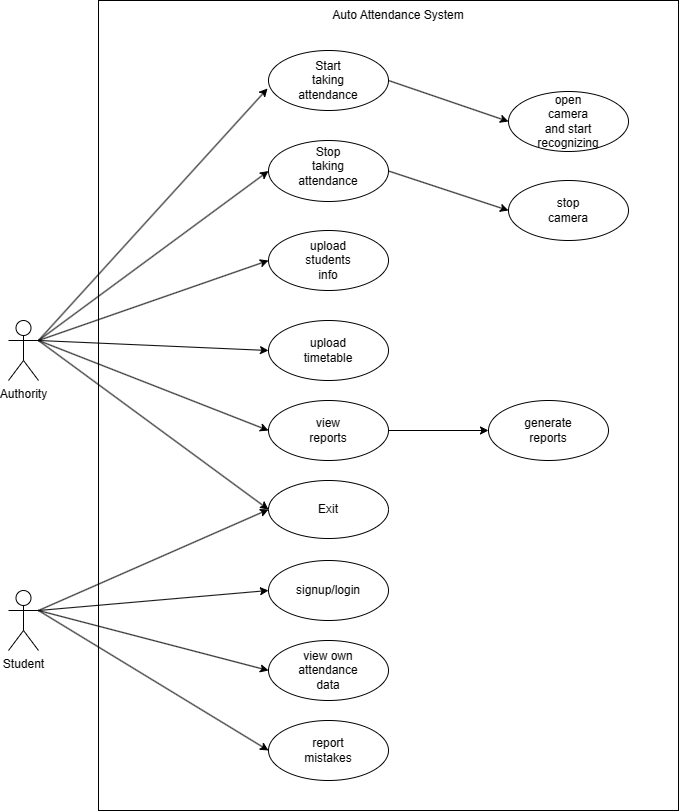
\includegraphics[width=\linewidth]{figures/use-case.png}
    \centering
    \caption{Use-case Diagram of the application}
    \label{fig:usecase}
\end{figure}

\subsection{Proposed Technologies}
Table \ref{table:tech} consists of the major technologies that are proposed to be used during the development and deployment of the application.

\renewcommand{\arraystretch}{1.5}
\begin{table}[H]
\centering
    \begin{tabular}{|l|l|}
        \hline
        \textbf{Subject}    & \textbf{Proposed Technology} \\ \hline
        Backend Database            & PostgreSQL           \\ \hline
        Backend Service    & Python        \\ \hline
        API Communication & WebSocket \\ \hline
        Frontend(Client)  & Next.js(React), Typescript, TailwindCSS              \\ \hline
        Deployment  & Docker Containers              \\ \hline
    \end{tabular}
    \caption{Technologies proposed to be used}
    \label{table:tech}
\end{table}

\subsection{Face detection algorithm}
We plan to utilize the OpenCV library in Python to train the model using students' images and detect faces for attendance purposes. We have two options for face detection: HOG + Linear SVM or MMOD CNN.\\

The HOG + Linear SVM face detector offers faster processing speed compared to the MMOD CNN method. However, it may be less accurate when dealing with changes in the viewing angle or rotation of faces.\\

For more robust face detection, we can employ the MMOD CNN face detector. This approach requires more computational resources, resulting in slower processing times. Nonetheless, it offers higher accuracy and is more resilient to variations in face rotation and viewing angles.\\

Furthermore, if we have access to a GPU, we can leverage it to run the MMOD CNN face detector, enabling real-time face detection. Combining the MMOD CNN face detector with a GPU delivers the perfect combination of deep neural network accuracy and the efficiency of a less computationally demanding model.\\

We have planned to use HOG + Linear SVM because of low resources and less time.\\

The HOG algorithm divides an image into small cells, computes each cell’s gradient orientation and magnitude, and then aggregates the gradient information into a histogram of oriented gradients. These histograms describe the image features and detect objects within an image.

\begin{table}[H]
\centering
\resizebox{\textwidth}{!}{%
\begin{tabular}{|l|l|l|}
\hline
\textbf{Algorithm} & \textbf{HOG + Linear SVM} & \textbf{MMOD CNN} \\
\hline
Approach & Histogram of Oriented Gradients (HOG) feature extraction & Convolutional Neural Network (CNN) \\
\hline
Training Complexity & Less computationally intensive & More computationally intensive \\
\hline
Speed & Faster & Slower \\
\hline
Accuracy & Less accurate, especially with changes in viewing angles & More accurate and robust to face rotation \\
\hline
Face Rotation Tolerance & Low & High \\
\hline
GPU Support & Limited (may not utilize GPU) & Utilizes GPU for improved performance \\
\hline
Model Size & Smaller & Larger \\
\hline
\end{tabular}%
}
\caption{Comparison of HOG + Linear SVM and MMOD CNN algorithms for face detection.}
\label{table:algorithm_comparison}
\end{table}

